\chapter{Nadajnik ultradźwiękowy}
\section{Budowa i zasada działania}

Nadajnik zbudowany został w oparciu o \textit{Arduino Nano} \cite{bib:arduinoNano} do którego podłączono 
bezpośrednio cztery nadajniki ultradźwiękowe (rezonatory piezoelektryczne) typu 40ST-12 \cite{bib:40ST12}, schemat 
przedstawiony jest na rysunku \ref{fig:nadajnik_schemat}.

\rysunek{transmitter}{schemat nadajnika ultradźwiękowego}{\label{fig:nadajnik_schemat}}


Całość umieszczona została w ramie w kształcie litery \textbf{H} wykonanej z rurek PCV.
Rezonatory zostały dodatkowo odizolowane od ramy rzepami co ułatwia ich zdejmowanie jak i skutecznie
zapobiega przenoszeniu się drgań.

\rysunek{nadajnik_H}{szkic ramy nadajnika}{\label{fig:nadajnik_szkic}}


Android Nano połączony jest z odbiornikiem 6m kablem, którym przesyłane są sygnały sterujące jak i zasilanie.
Do sterowania wykorzystywane są trzy przewody, dwa z nich informują który z rezonatorów ma w danym momencie nadawać,
trzeci służy jako wyzwalacz. 

Cała logika oprogramowania mieści się w obsłudze przerwania sprzętowego, które reaguje na zmianą stanu logicznego
na wyzwalaczu,
po uruchomieniu przerwania oprogramowanie wysyła sygnał na odpowiedni rezonator. 
Nadawany sygnał jest tak dobrany by dało się go w prosty sposób wyodrębnić i składa się w dwóch
części: część wzbudzającej oraz części tłumiącej.
Długość impulsów sygnału jest zgodna z częstotliwością rezonansową nadajników, dodatkowo część tłumiąca
jest przesunięty względem części wyzwalającej o 180 stopni.  
Rysunek \ref{fig:output_signal} przedstawia sygnał jakim wysterowany jest przetwornik piezoelektryczny. 

Odległość między nadajnikiem a odbiornikami wyznaczany jest przez odbiornik na podstawie
czasu jaki potrzebował sygnał dźwiękowy by do niego dotrzeć.

 \begin{figure}[h!]
    \centering
    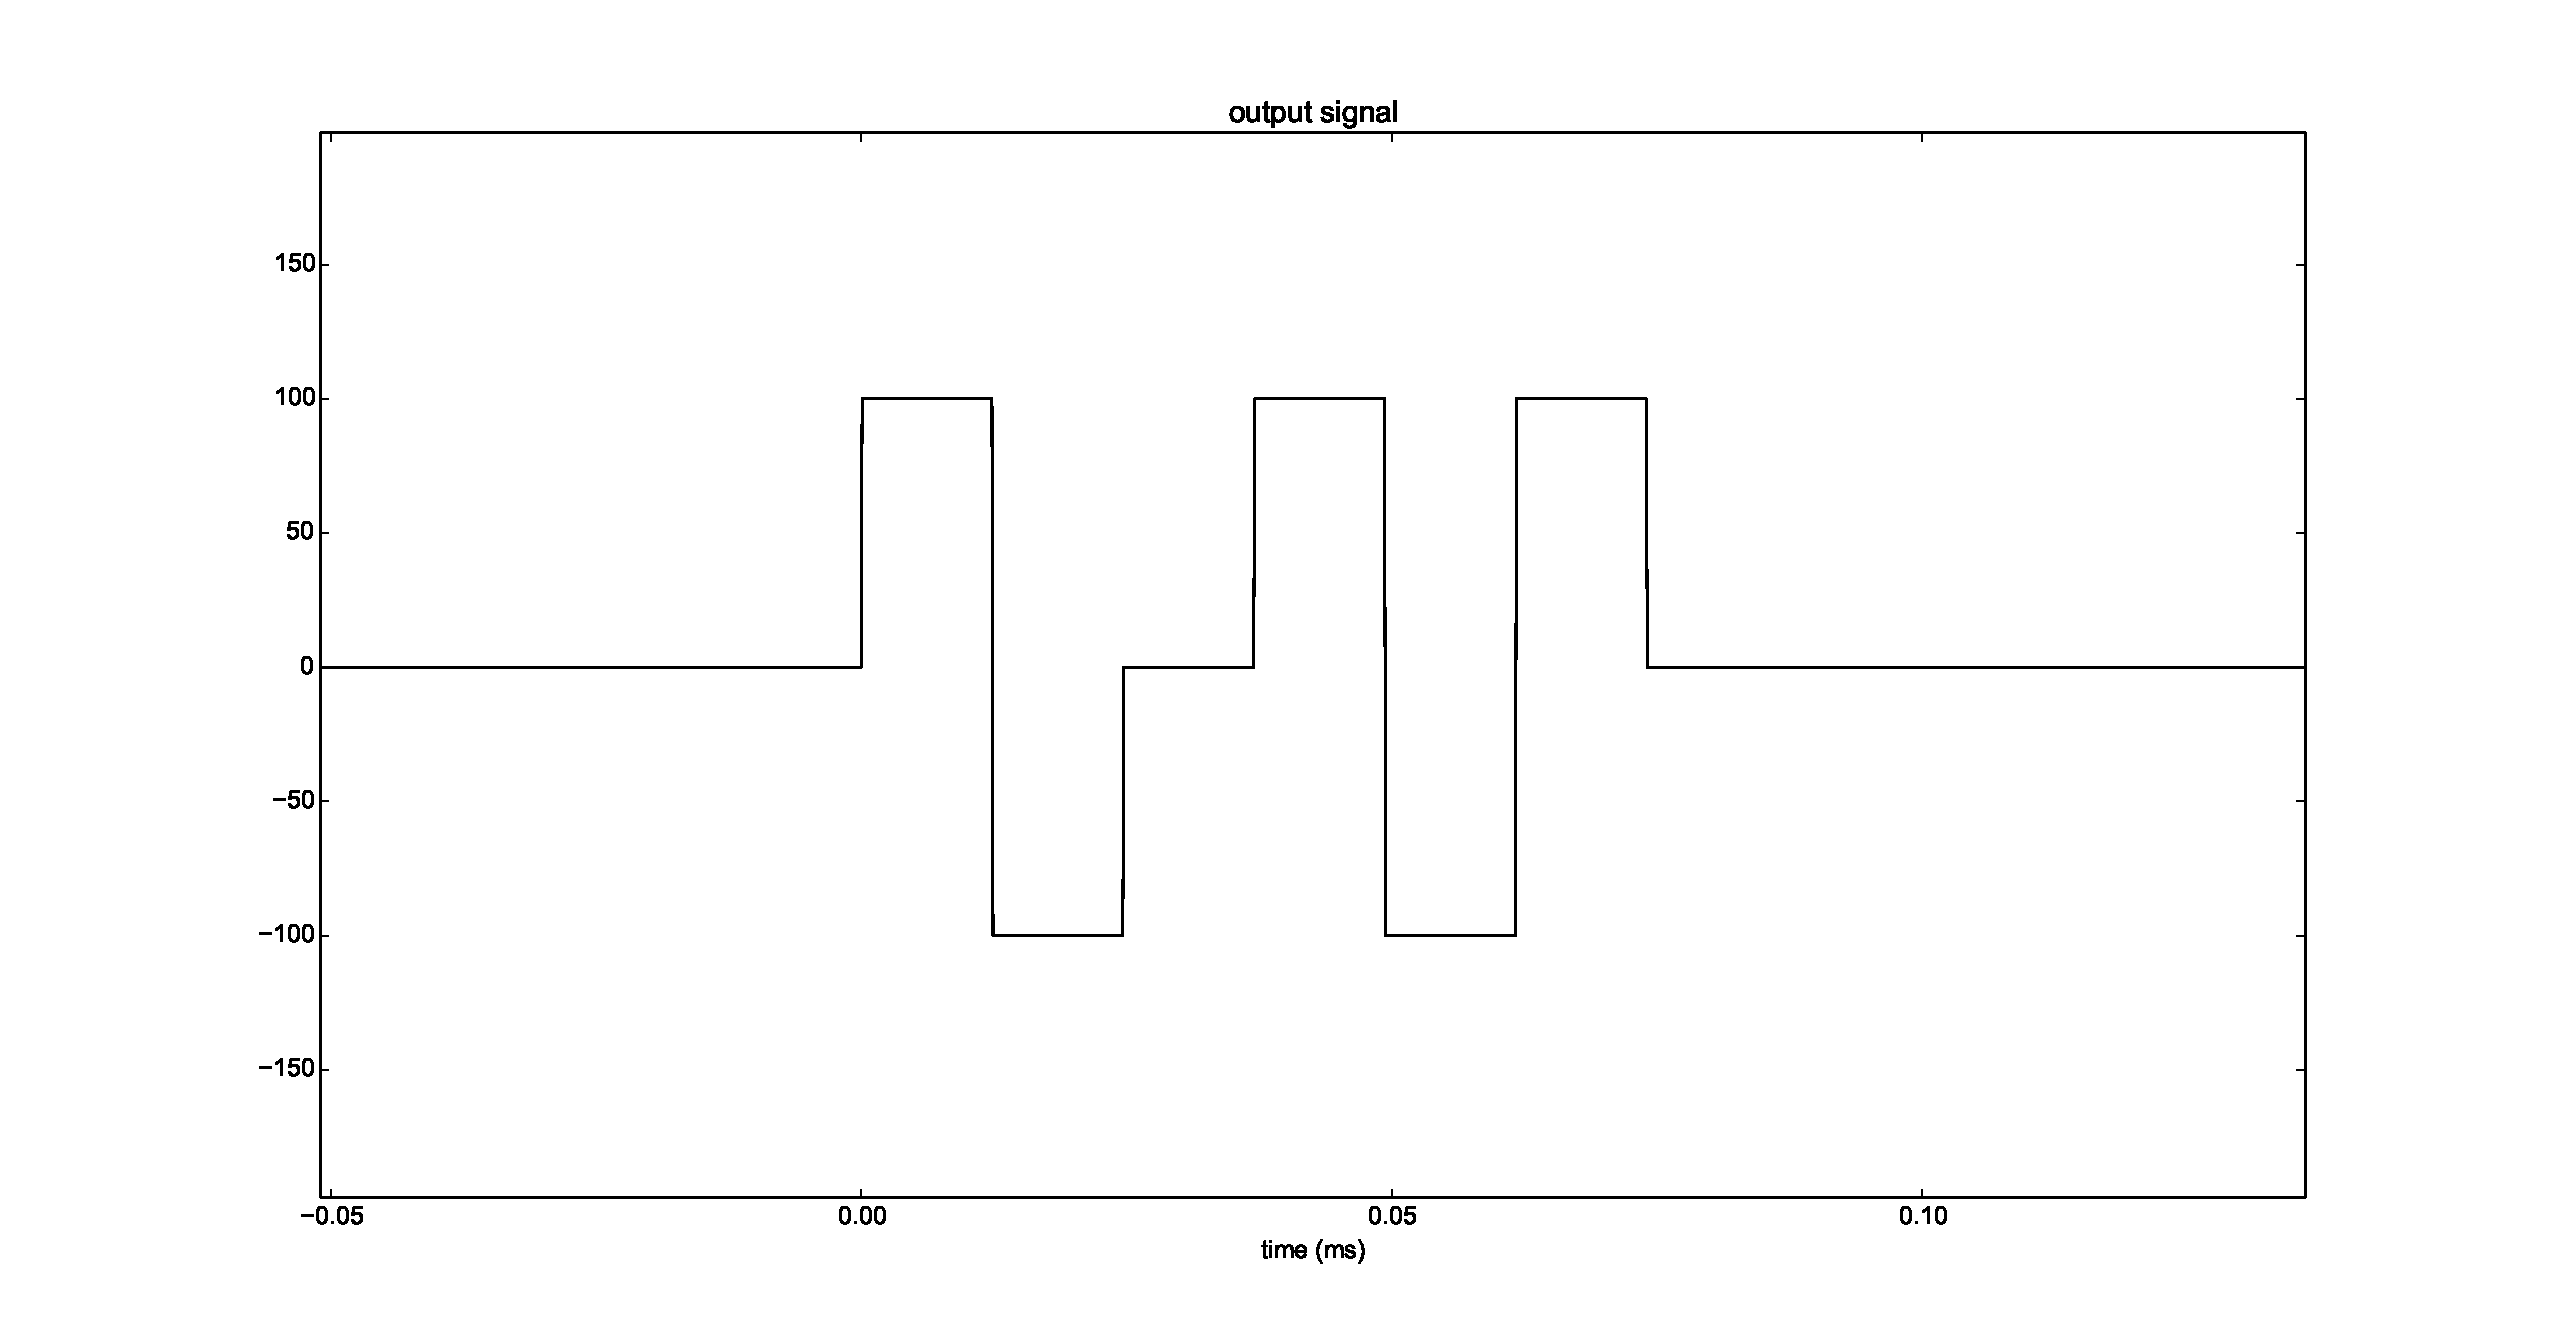
\includegraphics[width=1.15\textwidth, trim= 47mm 0mm 0mm 0mm,clip]{output_signal}
    \caption{sygnał wysterowania nadajnika piezoelektrycznego}
    \label{fig:output_signal}
\end{figure}

\newpage

\section{Dobór rezonatorów piezoelektrycznych}

Głównym problemem podczas konstrukcji nadajnika okazał się dobór odpowiednich rezonatorów piezoelektrycznych.
Mimo, że producent zapewnia zakres pracy rezonatorów w zakresie: $40 kHz \pm 1kHz$, taki rozrzut okazał się niewystarczający, 
dlatego z 30 rezonatorów (15 nadajników i 15 odbiorników) wybrane zostały 4 nadajniki i 3 odbiorniki o najbardziej 
zbliżonych częstotliwościach pracy. Częstotliwości zostały zmierzone na oscyloskopie cyfrowym, są to odpowiedzi 
rezonatora na krótki impuls elektryczny.

Tabela \ref{table:czestotliwosci} zawiera wyniki pomiarów częstotliwości, gwiazdką oznaczono wykorzystane przetworniki piezoelektryczne.

\begin{table}[t]
  \centering
  \begin{tabular}{|r|r|r|}
    \hline 
    nr & nadajnik: 40ST-12 & odbiornik: 40SR-12\\
    \hline
    1  &   40.88kHz & *40.65kHz \\
    2  &   41.12kHz &  40.45kHz \\
    3  &  *40.78kHz &  39.52kHz \\
    4  &   41.19kHz &  40.47kHz \\
    5  &   40.92kHz &  40.66kHz \\
    6  &   39.68kHz & *40.69kHz \\
    7  &   39.78kHz &  40.59kHz \\
    8  &  *40.80kHz &  40.39kHz \\
    9  &   40.90kHz &  40.29kHz \\
    10 &  *40.66kHz & *40.68kHz \\
    11 &  *40.85kHz &  39.22kHz \\
    12 &   41.01kHz &  39.51kHz \\
    13 &   41.00kHz &  39.92kHz \\
    
    14 &   39.82kHz &  39.26kHz \\
    15 &   39.64kHz &  39.11kHz \\
    \hline
  \end{tabular}
  \caption{Częstotliwości rezonansowe przetworników piezoelektrycznych}
  \label{table:czestotliwosci}
\end{table}


